%% This is an example first chapter.  You should put chapter/appendix that you
%% write into a separate file, and add a line \include{yourfilename} to
%% main.tex, where `yourfilename.tex' is the name of the chapter/appendix file.
%% You can process specific files by typing their names in at the 
%% \files=
%% prompt when you run the file main.tex through LaTeX.
\chapter{Overview of Visual-inertial Odometry}
\label{chap:Overview}

In this chapter, we will overview our visual-inertial odometry system. In section \ref{sec:notations}, we first introduce the world representations (\eg, world frame, camera frame and IMU frame) together with basic notations in our odometry system. In section \ref{sec:FVK}, we then discuss two important schemes, filter method and keyframe Bundle Adjustment(keyframe BA) in SLAM algorithm, and explain why we finally choose the keyframe-based method.

\section{World Representations and Notations}
\label{sec:notations}

\begin{figure}[h]
    \centering
    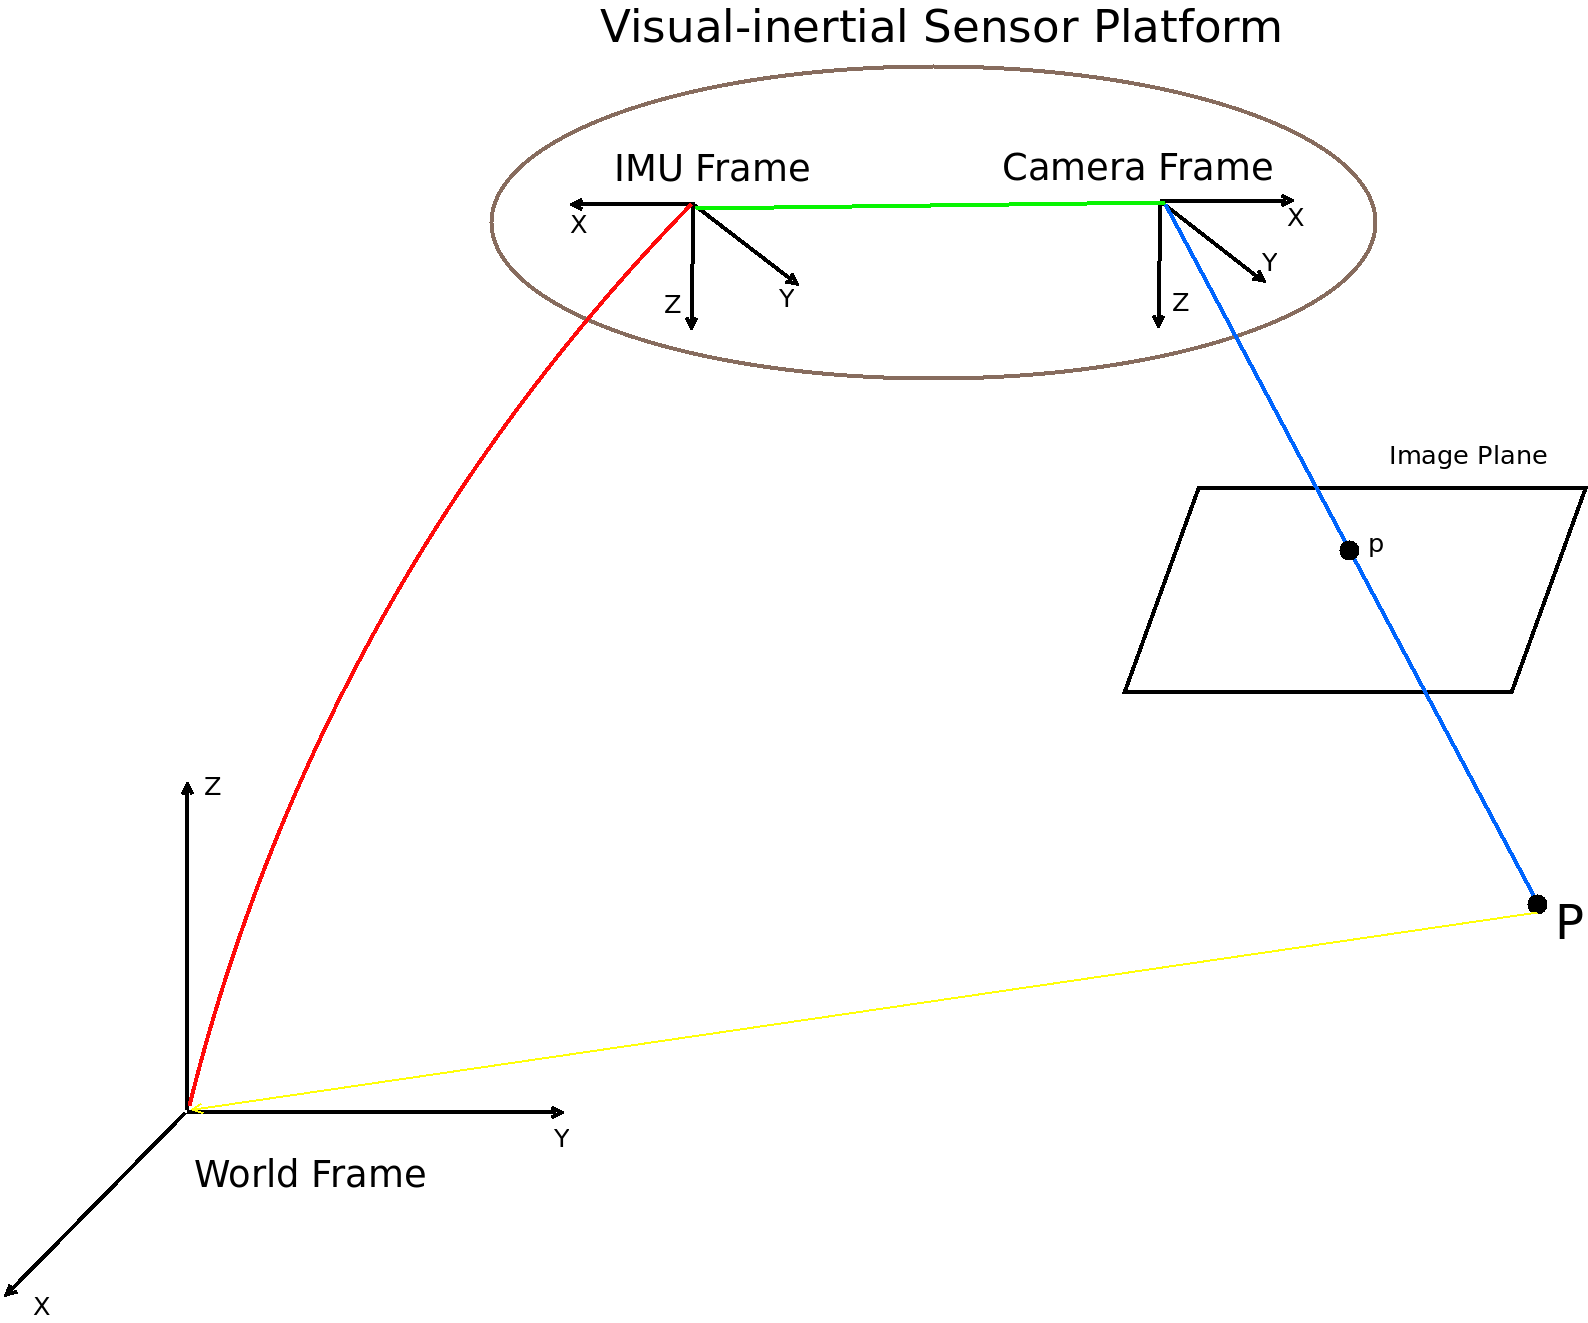
\includegraphics[width=0.8\textwidth]{CONTENT/Figure/Figure2-1_World.png}
    \caption{This figure shows the connection among the world frame $\W$, the IMU frame $\I$ and the camera frame $\C$. Green line shows the transformation between the camera and IMU, which can be pre-calibrated. Red line is the pose of IMU in the world frame. The camera frame observes point $\textbf{p}$ of object P in the image plane, and it connects a object P by blue line. The coordinate of object P in the world frame is presented as yellow line.}
    \label{fig:fig2-1}
\end{figure}

Visual-inertial odometry (VIO)~\cite{li2011consistency}, literally, is an odometry system, which receives environment information by visual (camera) and inertial (IMU) sensors. VIO is similar with the well-known visual odometry (VO) problem \cite{nister2004visual}, with an additional IMU sensor. VIO tries to estimate agent's pose while the agent moves in the environment. One major difference between odometry and SLAM algorithm is that odometry system usually does not build a map \cite{li2011consistency}, whereas SLAM algorithm simultaneously localizes and constructs a map.

To setup a VIO system, we need to first define the world representations. Globally, we have a world frame $\W$; world frame $\W$ is set to a right-handed Cartesian coordinate system that every objects has an absolute pose (translation and rotation). Each sensor has its own local frame, \ie, IMU frame $\I$ and camera frame $\C$, which is also defined as a right-handed Cartesian coordinate system. Every time sensors obtain observations within their own local frame, we estimate the pose of those sensors in world frame $\W$ by integrating these measurements over time. Figure \ref{fig:fig2-1} shows the overall world representations, and connections between different frames.

In this master thesis, we mainly use following notations,
\begin{itemize}
\item {We denote scalars as $a, b, c$, vectors as $\textbf{a}, \textbf{b}, \textbf{c}$, matrices as $\mA, \mB, \mC$, and frames as $\A, \B, \C$.}
\item {We denote a measurement $\textbf{m}$ in a particular frame $\F$ as $\textbf{m}_{\F}$. To further simplify, any parameter that is \textbf{not} in the world frame will be denoted particularly. For example, the translation $\textbf{p}$ in the camera frame will be denoted as $\textbf{p}_{\C}$, and the translation $\textbf{p}$ in the world frame will be simply denoted as $\textbf{p}$. }
\item {A general translation $\textbf{t}$ should express a translation from point $A$ to point $B$ in frame $\C$, which is hereby denoted as $\textbf{t}^{AB}_{\C}$. In order to simplify our notations, we denote a point $\textbf{p}$ in frame $\A$ as $\textbf{p}_{\A}$ if this point is the translation $\textbf{t}^{OP}_{\A}$, where $O$ is origin of frame $\A$, and $\textbf{p} = P$. This holds same for vectors, which means we can directly use a point $\textbf{p}$ to represent a vector from origin to $\textbf{p}$.}
\item {A general rotation is either expressed in a quaternion $\textbf{q}$ or a rotation matrix $\mR$. To clarify our notations, here we use quaternion $\textbf{q}$ as an example. A quaternion is an orientation operation from frame $\B$ to frame $\A$, and it is denoted as $\textbf{q}_{\A\B}$  in this thesis. Note that if such a operation is from world frame $\W$ to a certain frame $\B$, we omit both frames for simplification, \ie, $\textbf{q}_{\B\W} \triangleq \textbf{q}$. These notations hold same for rotation matrices.}
\item {We use hat operator to represent the estimation of state, \ie, $\hat{\vec{x}}$ is the estimation of state $\vec{x}$.}
%TODO: Add more notations when necessary
\end{itemize}

\section{Filter Versus Keyframe}
\label{sec:FVK}

\begin{figure}
\centering
	\begin{subfloat}[Filter]{
		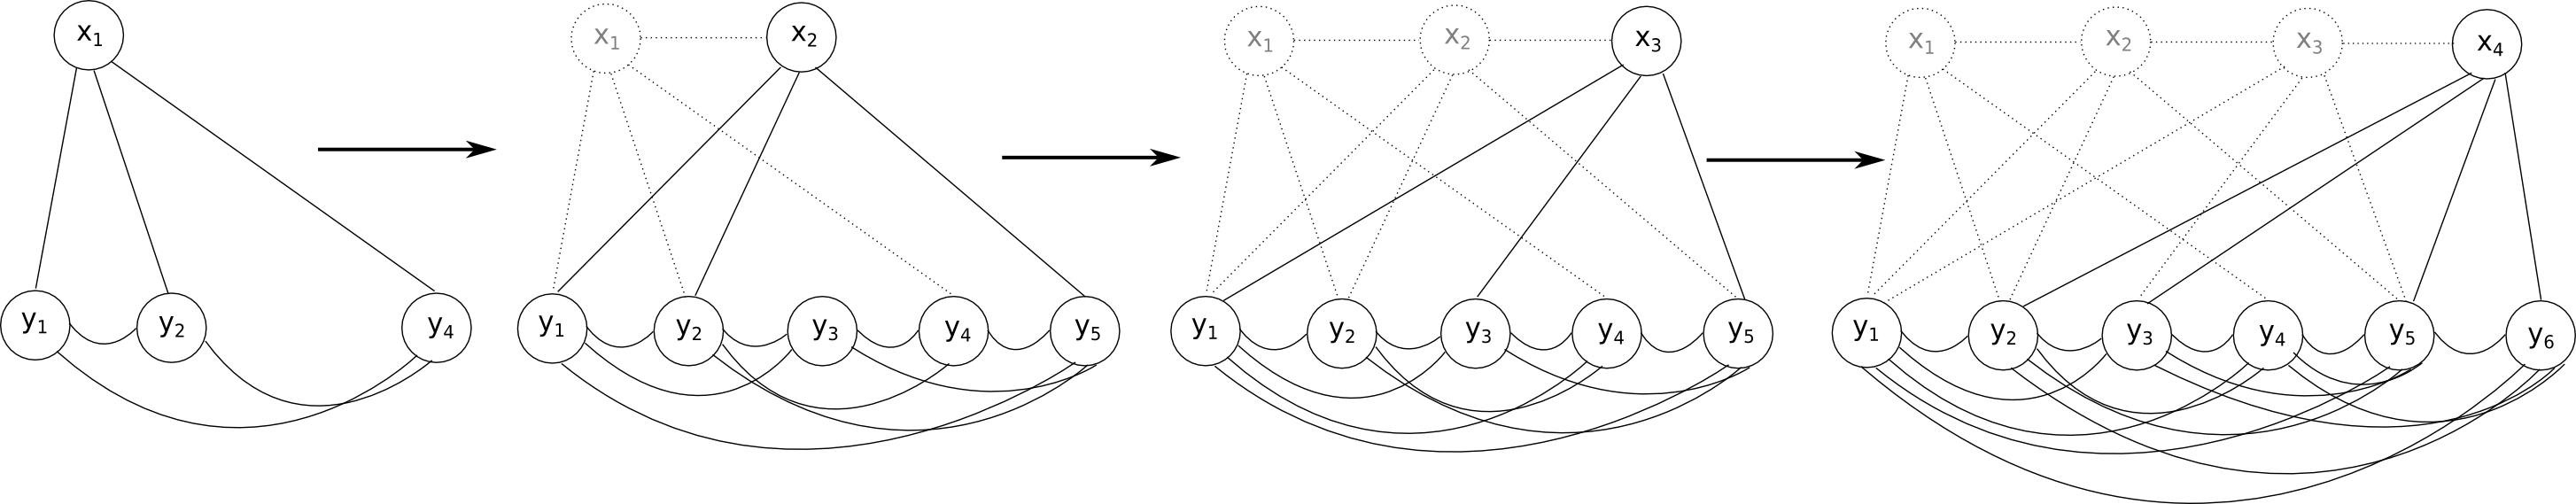
\includegraphics[width=1.0\textwidth]{CONTENT/Figure/Figure2-2-a.png}
		\label{fig:fig2-2-a}}
	\end{subfloat}
	
	%\hspace*{\fill} % separation between the subfigures
	
	\begin{subfloat}[Keyframe-based BA]{
		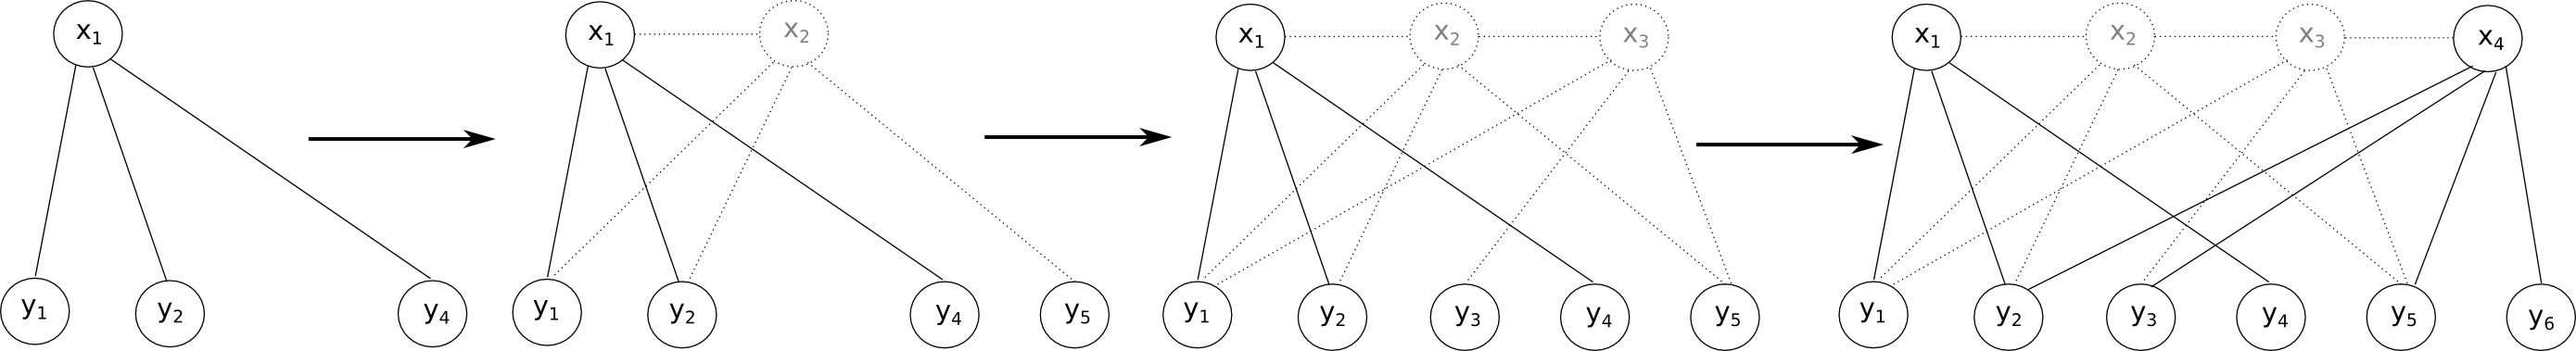
\includegraphics[width=1.0\textwidth]{CONTENT/Figure/Figure2-2-b.png}
		\label{fig:fig2-2-b}}
	\end{subfloat}
	
	%\hspace*{\fill} % separation between the subfigures
	
	\caption{(a) Filter method for SLAM. (b) Keyframe-based Bundle Adjustment (BA) for SLAM. We denote the $i^{th}$ camera position as $\vec{x}_i$,  $i^{th}$ image feature as $\vec{y}_i$. We connect the line between camera and image feature if this feature is observed by this camera, the vanished observations is presented as dotted line, and the vanished camera is expressed as grey font. Both graph changes as time goes on from left to right. From (a) one can see that though only the latest camera pose is reserved, the number of edges between features are increasing fast. (b) stores some previous camera poses (keyframe) (\ie, $vec{x}_1$ and $\vec{x}_4$), thereby keeping the graph sparse. } 
	\label{fig:fig2-2}
\end{figure}

It is important to note that though this thesis focuses on visual-inertial odometry for small workspaces, we intend to keep the possibility to extend our system to a general, scalable, and efficient SLAM system as well. Therefore we briefly introduce the basic concepts of SLAM here. SLAM system usually has two parallel processes, one is for localization and another is for mapping, the crucial point of building such a system is to keep both processes efficient. There are two general frameworks in visual SLAM: filter-based method and keyframe-based method. In this section, we will discuss whether filter-based method or keyframe-based method is more suitable for our case.

Filter-based SLAM \cite{davison2007monoslam, eade2007monocular, davison2003real} uses \textit{extended Kalman filter} (EKF) to propagate states and update the state covariance matrices. In each step, the system obtains the current estimation of camera pose and landmark positions (3D points) by marginalising previous camera poses. This marginalization step usually eliminates the former pose and adds a few more connections to image features. As shown in Figure~\ref{fig:fig2-2-a}, the size of graph will not grow very fast as time flows, since the former pose has been eliminated and features in environment is limited. However, once the system moves to large scale scene, it will consume more time to optimize the poses and landmarks as the graph tends to be fully-connected. 
   
Keyframe-based SLAM \cite{klein2007parallel, mourikis2007multi, forster2014svo, engel2014lsd, mur2015orb} applies \textit{bundle adjustment} (BA) on keyframes to update the map. In keyframe-based SLAM, it stores some historical poses (keyframes) and image feature points to proceed a BA step. The chosen of keyframes varies from different implementations, and the idea is to choose a frame that is not very close to the last keyframe to avoid redundant information. From Figure~\ref{fig:fig2-2-b}, it is clear that the graph stays sparse as the number of poses and features increases. Another benefit for the keyframe-based approaches is that it is more convenient to handle loop closures since the historical camera poses have been preserved.

In \cite{strasdat2010real}, they have shown that the computational cost for keyframe BA is $O(m^2 \cdot n)$, and for filter method is $O(n^3)$, where $m$ is the number of key frames, and $n$ is the number of landmarks. They conclude that keyframe-based SLAM is slightly better than filter-based SLAM with their experiment settings, especially when scale of scene becomes larger so that the number of landmarks is far more larger than the number of keyframes. 

In this master thesis, we choose keyframe-based method for the visual part and filter method for the IMU integration part. Since we do not keep former information (\eg, image features or landmarks) in integration step, filter method is more efficient whereas each filter step can be regarded as an single optimization step. The reason that we use keyframe-based method for visual part is that we intend to improve the scalability of our system. Moreover the results from IMU integration are a good compensation to visual SLAM since the output frequency of IMU sensors is usually higher than visual sensors.

